\section{Results}

\subsection{Results}

The circuit obtained in the previous section can be applied to a system of 4 qubits several times to perform a random walk. 
Fig. 2 shows the results of a 100 steps random walks, obtained by apply the circuit 100 times. 

\begin{figure}[h!]
    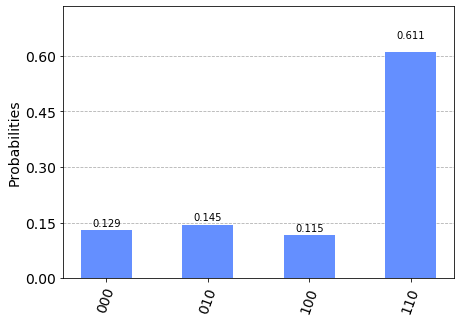
\includegraphics[scale=0.4]{img/100_steps_walk.png}
    \caption{results of a 100 step random walk}
    \centering
\end{figure}

As we can notice in the picture the probailities of find the walker in a given position are 
quite asymmetrical and also since we started from an even number, odd numbers have zero probability of 
being measured, in fact, differently from classical, we can 
see a true randomness behavior different from a Gaussian distribution that we will obaserve in a 
classical random walk. The image belowe taken from \cite{Kendon2004} shows a comparison between
the gaussian distribution of classical systems and the distribution observed for the quantum after 
100 step of the walk.

\begin{figure}[h!]
    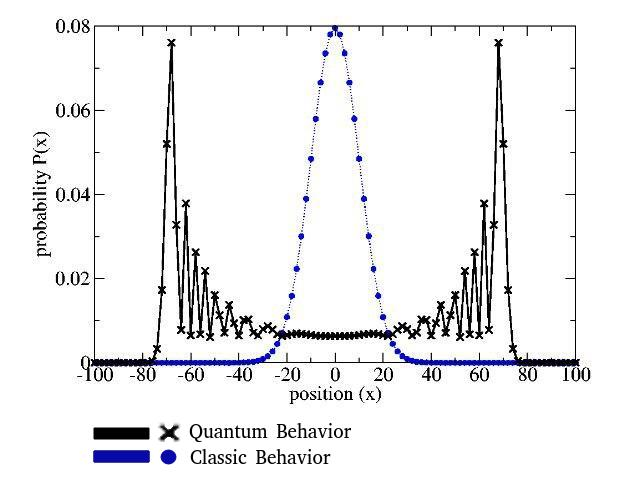
\includegraphics[scale=0.5]{img/dist.jpg}
    \caption{comparison of distribution of a 100 step random walk between classical and quantum}
    \centering
\end{figure}

This means that the walker can pass through or be in an odd(even) but the probability to measure the Walker in a odd(even) position starting 
from an even(odd) position after 100 steps of the walk is very close to zero.  
This strange behavior is due to the Hadamard coin, this coin treats the two direction (left, right) differently, 
considering the two states $\ket{\uparrow }$ and $\ket{\downarrow }$ this coin multiply the phase 
by -1 only in case of $\ket{\downarrow }$ inducing more cancellations of the right-wards paths. \cite{Kempe_2003}

The asymmetrical behavior can be modified by changing the initial state or 
changing the coin or balance the Hadamard coin, a more formal description of this behavior is showed in \cite{6812670}.

This particular distribution is interesting since shows that quantum can achive a true randomness, classical computer
can only simulate a random behavior, for sure useful and well done, but still simulated. 